\documentclass[11pt]{article}

\usepackage{graphicx}
\usepackage{float}
\usepackage{listings}
\usepackage{amsfonts} 
\usepackage{amsmath}
\usepackage{amssymb}
\usepackage{placeins}
\usepackage[dvipsnames]{xcolor}

\usepackage[no-math]{fontspec} 
\setmainfont{Times New Roman}

\usepackage{hyperref}
\hypersetup{
    colorlinks=true,
    linkcolor=blue,
    filecolor=magenta,      
    urlcolor=cyan,
}

\definecolor{commentgreen}{rgb}{0.0, 0.5, 0.0}

\lstset{
  language=C,
  basicstyle=\footnotesize\ttfamily,
  numbers=left,           
  numberstyle=\tiny,       
  tabsize=5,                 
  extendedchars=true,         
  breaklines=true,
  commentstyle = \color{commentgreen},
  keywordstyle=\color{blue}\textbf,           
  stringstyle=\color{white}\ttfamily,
  showspaces=false,       
  showtabs=false,           
  showstringspaces=false,
  morekeywords={procedure, foreach, in}
}

\newcommand{\classname}[1]{\textit{\textbf{#1}}}
\newcommand{\varname}[1]{\underline{\textit{#1}}}
\newcommand{\funcname}[1]{\textit{#1}}

\title{
  ICS2211 Assignment \\
  \large Team \#8, life below water
}
\author{Lorenzo Catania, Malcolm Grech, Francesco Borg Bonello}

\begin{document}

\begin{titlepage}
\begin{figure}
  \centering
  
\includegraphics[width=1.0\textwidth]{figures/frontpage}
\end{figure}
\end{titlepage}

\maketitle

{
  \hypersetup{linkcolor=black}
  \tableofcontents
}

\section{Introduction}
\subsection{Game concept}
The presented project is a side-scrolling arcade game called \textbf{Deep Blue}, set in a fictional underwater world where the sea-life had become accustomed to the garbage dumped in the ocean, enough that they become genetically mutated and start living off of it. The player embodies a scuba diver that needs to collect as much rubbish as possible while evading these mutant sea creatures.

\subsection{Game mechanics}
The game is a side-scrolling runner, where the world is discovered from left to right, with the camera scrolling only to the right. The player must collect as much rubbish as possible (represented as cans, plastic bags, plastic bottles and other classical illustrations of rubbish) to increase the score. Enemy fish are periodically spawned and start patrolling different areas of the screen. If the player approaches an enemy for too long, then it becomes aggroed and begins targeting the player. The player does not attempt to defeat the enemies, but rather evades them (they do despawn once out of the map’s range however).

The player must take care of the available oxygen level, which gradually drops while underwater and can be replenished by resurfacing. The rate of this drop is based on the character depth. Once out of oxygen, the player begins losing health.

The player may find power-ups in the map or inside rubbish. These are useful to the player by healing, recovering oxygen or permanently increase speed to make it easier to run away from enemies.

The environment is procedurally generated, meaning that each game may be potentially infinite. Items, collectables and enemies are spawned randomly, which are then despawned when falling off the left of the screen. These enemies’ strength grow over time and have a small chance to evolve to a more dangerous kind of organism.

\section{Software architecture}
\subsection{Development environment}
The game has been developed using Unity3D 2018.4.13f and has been tested on both Windows and GNU/Linux operating systems. No specific versioning control software was used, but it’s possible to reconstruct a rough history of the code since each proposed change was packaged into a Unity Package, uploaded on google drive and imported by the rest of the team after carefully testing.

\subsection{Components}
\subsubsection{Level generation}
The ‘LevelGenerator’ is responsible for spawning collectables and any neutral entity the player can interact with in general. It contains a list of prefabs with their respective probability of spawning and the range of coordinates they spawn. The level generation happens in an area on the right side of the camera that’s still not visible to the player. This area is split into tiles of fixed sizes and are filled with entities that are then attached to the root node of the scene so that they can shift on the left and interact with the current game environment. Two entities spawned in the same update cannot appear in close tiles to guarantee world variety. Note that enemies may have been spawned by this level generator, but where not implemented in the final version of the game since a more dynamic way of evolving had been preferred. In fact, game objects spawned by the level generator are initialized in-place and deallocated when their lifecycle finishes. This approach doesn’t affect the performance of simple objects, but may limit the versatility of highly intelligent” ones such as enemies.

\begin{figure}[H]
  \centering
  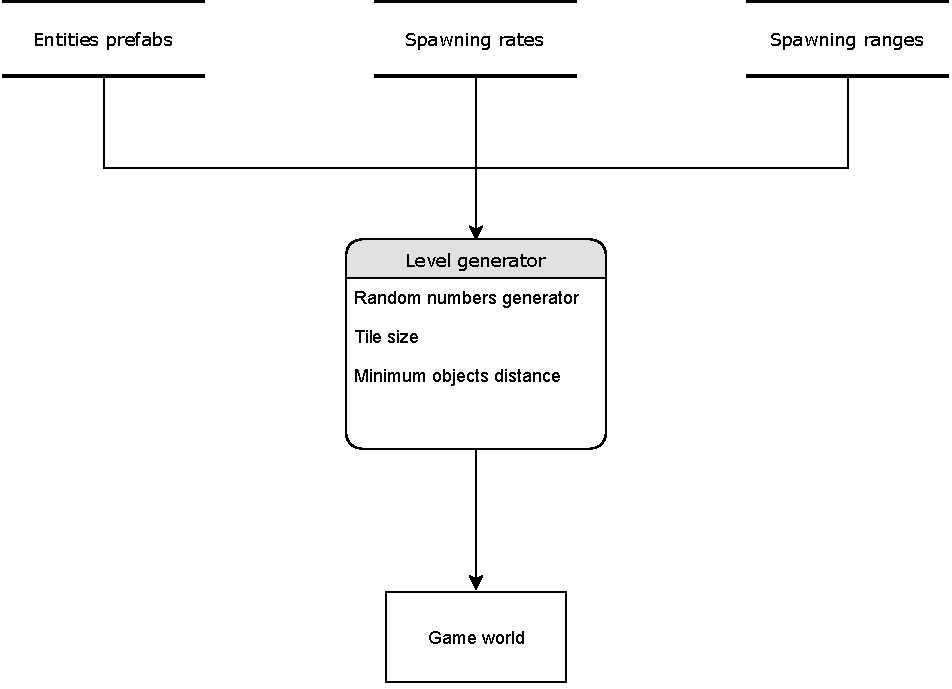
\includegraphics[width=1.0\textwidth]{figures/level_generator}
  \caption{Level generation data flow}
\end{figure}

\subsubsection{Camera movement control}
The ‘CameraController’ component handles the main camera movement and the appearance of visual details in the scene.

The camera smoothly follows the player movement, but is clamped on the vertical axis to prevent showing the void behind the background sprite. The camera moves slightly faster on the horizontal axis based on how close the player is to the right bound of the screen.

As the player object moves in the scene world, the background image must be continuously shown and moved forward, without letting the player notice the loop.

Two seamless background textures are loaded and put side by side. When the leftmost one leaves the camera’s visual, it is translated to the right of the other recursively. In doing so, the player will never see the void behind the background while also preserving performance in the long run as the only operation done is a casual translation rather than constant generation.

\begin{figure}[H]
  \centering
  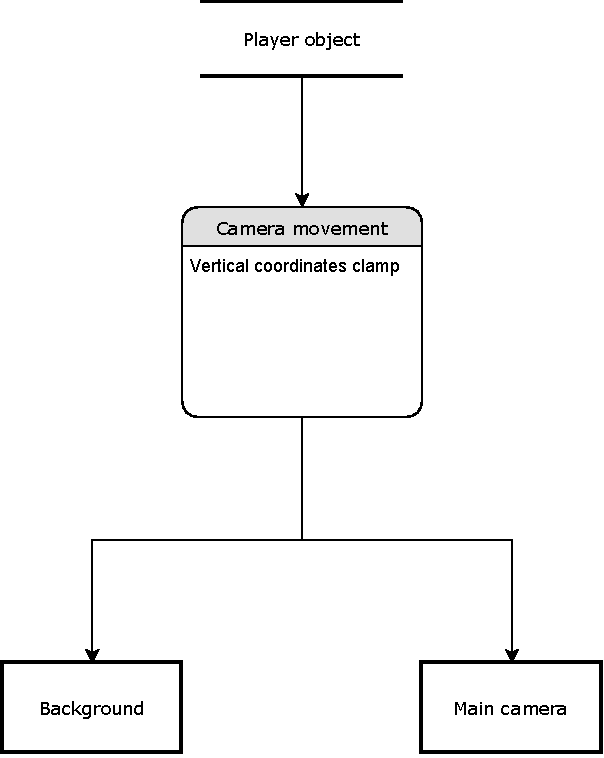
\includegraphics[width=0.8\textwidth]{figures/camera_controller}
  \caption{Camera control data flow}
\end{figure}

\subsubsection{Player control}
The player object is controlled by always moving towards the cursor where the speed is adjusted based on its distance from the player object. The rotation is also delayed to simulate the underwater physics effect. Furthermore, the head movements are faster than the body movement and hence looks at the mouse pointer much faster to give a better idea of where the player will go.

Player’s health and oxygen values are also handled by a script, mainly to determine the point at which its “game over”. External entity interactions (such as enemies and collectables) may change these values as well. The player position is checked at every update loop to determine whenever oxygen is gained or spent based on the depth (represented by the player’s position in the Y axis).

Raycasting is used all around the player object to see if any collectable is present, and if it may be picked up. 

\begin{figure}[H]
  \centering
  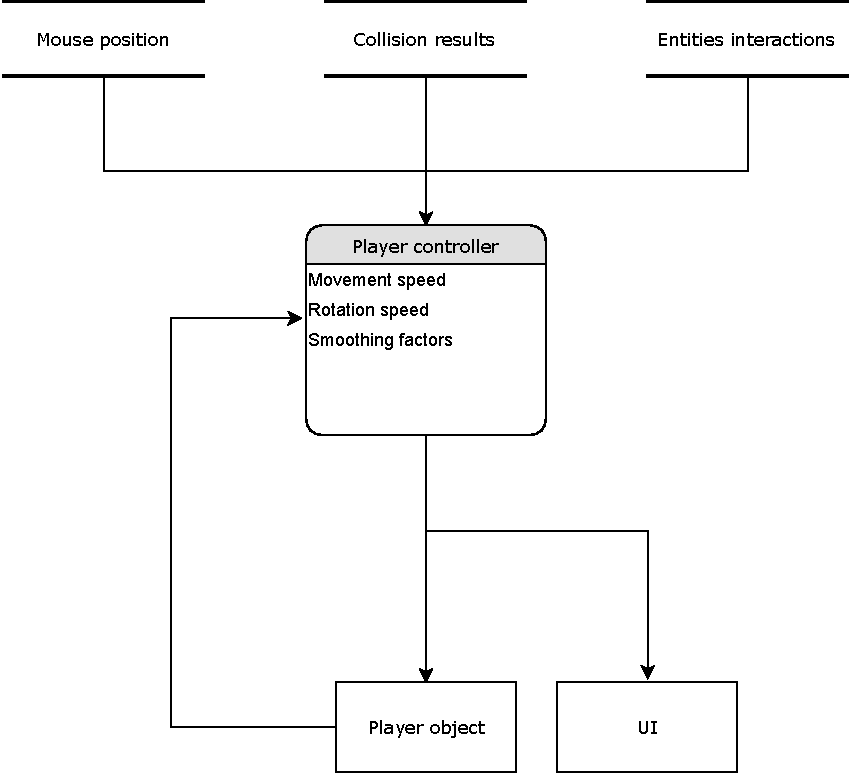
\includegraphics[width=1.0\textwidth]{figures/player_controller}
  \caption{Player control data flow}
\end{figure}

The backward arrow between the player object and its controller represents the usage of current player data (such as the position) to compute what values should be present in the next step.

\subsubsection{Player survivability}
Survivability is a very important aspect of this game as it determines how long a single playthrough will last given that the level is infinitely generated. Two factors were adopted in this game via a script that handles both: Health and Oxygen Levels.

Regards to health, the player starts with 100 health points which gets reduced when attacked by an enemy, with the amount of damage done is based on the enemy’s stats. The Oxygen Level decreases over time, based on how deep the player is below sea-level. Thus, if the player dives to the seabed, they would lose Oxygen at a much faster rate than if they were located near the surface of the sea. When the level of oxygen reached zero, the player starts to lose health points until eventually dying and ending the game.

The above were displayed to the user via UI at the top-left of the screen in the form of a slider bar.

\subsubsection{Pickups and powerups}
Each garbage pickup has the chance to spawn a powerup which the player must react quickly to change their direction and catch it before it floats away.

Powerups are randomly spawned throughout the level. These powerups are: Health; Oxygen; and Speed Boost.

The health pickup adds 20 points of health when picked up, while oxygen pickup adds 50 points of oxygen to the players oxygen level. The speed buff increases the overall speed of the player permanently.

\subsubsection{Entities garbage collection}
A ”death wall” object was placed on the left of the screen and moves with the camera. It has a trigger which collides with all the game objects (expect the back-ground image). Each time an object is far enough from the user’s point of view it is deleted or sent back to its relative pool to optimize memory usage and clean the scene from useless objects that no-longer need rendering.

\subsubsection{Game state and UI}
In the current version, the game state is given only by the score. A \textit{‘ScoreManager’} is used to keep track of its value and to update the score’s label on the GUI.

Menus are composed by buttons that interact with a \textit{'ButtonHandler'}, calling different function based on what action must be executed (which generally load a different scene). In-game user interface is made of icons a slider, or texts that represents the player stats and the current user score. These are also updated by controller. A more in-depth analysis on the menu system is contained in the next section.
The usage of anchoring was vital to keep all the information in the correct areas of the screen when playing on screens of different sizes.
The approach taken was to keep a minimalistic amount of text and instructions on the screen, hence the reason that we didn’t use the text of ‘Score’ to notify the player that that was the score they have, but instead used an generic image for garbage. Therefore, this nudge urged the player to pick up garbage. In the same way, the health bar was represented with the symbol of health (a green ‘+’ sign) and the oxygen level represented by the players oxygen tank.

\subsubsection{Menu interface}
The game menu had been designed with functions that are global throughout all scenes, such as the ability to go to the settings when pressing escape/ pausing, and initially with a single soundtrack until it was decided to have different sounds for each scene. This was done by the player loading into a master scene to load these functions, then directly to the ‘mainMenu’ scene.

With an option of 3 buttons, the player may begin playing, go to the setting scene, were sound may be adjusted, or terminate the program. When pressing ‘Escape’ or ‘Enter’ at any point while in the main menu or in gameplay, the settings scene may be loaded. By pressing one of them again the player may return to their previous scene, or do so by means of another provided button. When in the settings scene, the player may adjust the volume of the soundtrack, and while not implemented, a pause feature had been in development to be included with this scene.

\begin{figure}[H]
  \centering
  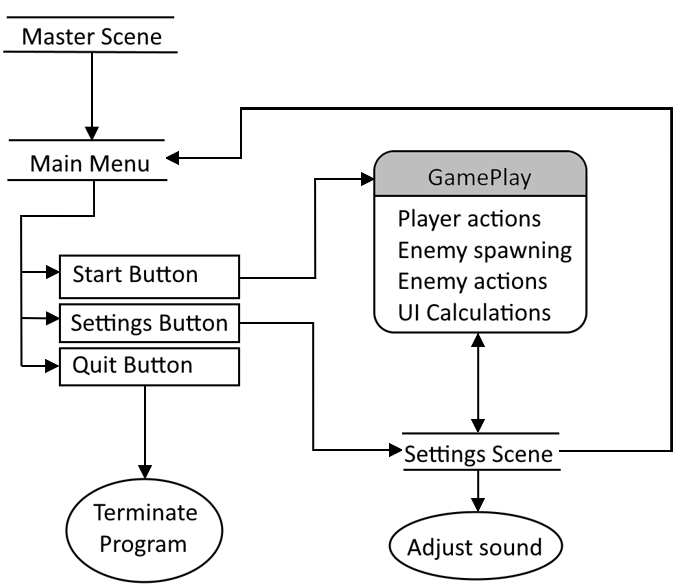
\includegraphics[width=0.6\textwidth]{figures/menu_system}
  \caption{Menus data flow}
\end{figure}

\subsubsection{Animations}
Our allocated graphics designer designed the requested sprites accordingly. For animations, they drew the sprite in multiple frames where we imported the file on unity and spliced it into different sprites. After minor tweaks such as the rate of frames per second in the animation and adjustment of sizes, the animation was displayed appropriately in game.

Our player was animated so as to be seen moving. The enemy shark was also animated in a similar way. Another indirect method of animation that was implemented is that the player sprite flashes in a red colour when damage is taken so to notify the player that they are in danger.

\subsubsection{Sound}
Sound played an important aspect in our game. These served as nudges to the player, for example when drowning from lack of oxygen, the player can hear the sound of someone drowning so as to cause a sense of panic and urge them to take the necessary measures to survive. A similar situation arises when the player is attacked by the enemies. A sound is also played upon the death of a player.

The background music enticed the underwater-spooky feel to the game. The main menu theme composed by one of our own members highlighted this by getting the player into the feel of the game. All other sounds were found online but edited by us before implementing into the game.

\subsubsection{Enemies spawning}
The model used to spawn enemies in the game world is unique and tuned specifically for gradually increasing the match difficulty. It’s based on a genetic algorithm, applied to a pool of pre-instantiated enemy objects that are partially destroyed and initialized again during the breeding phase.

Enemies in the pool are bred periodically, and a new enemy is popped out from the pool and spawned in the world. Note that enemies currently present in the scene are not involved in breeding, so the process is completely invisible to the player.

Different kind of enemies can be encountered while playing, and the variety is guaranteed by mutations during reproduction of enemies. This means that a child may mutate to a different species instead of inheriting its genes from the parents. Thus, the chance of encountering weaker species decreases over time.

The approach used to breed enemies is described in further detail in the next section.

\begin{figure}[H]
  \centering
  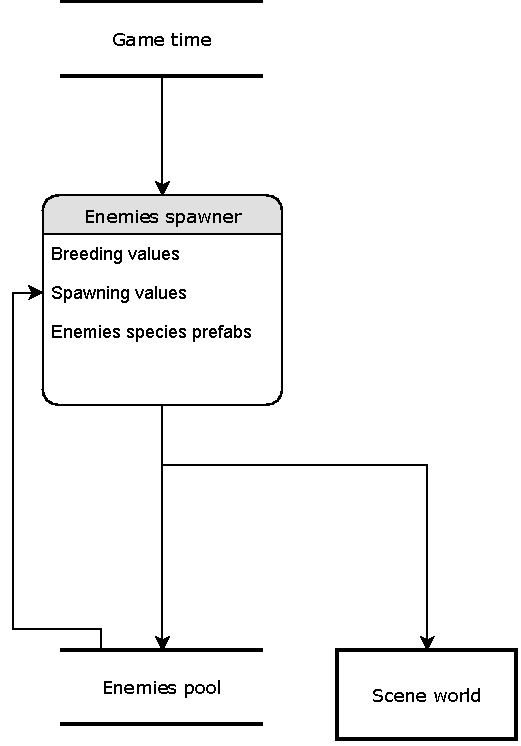
\includegraphics[width=0.6\textwidth]{figures/enemies_spawner}
  \caption{Enemies spawner data flow}
\end{figure}

\section{Artificial Intelligence features}
\subsection{Enemies behaviour state machine}
The enemies' behaviour is traced by a simple finite state machine that contains two states: \classname{patrolling} and \classname{attack}.

\begin{figure}[H]
  \centering
  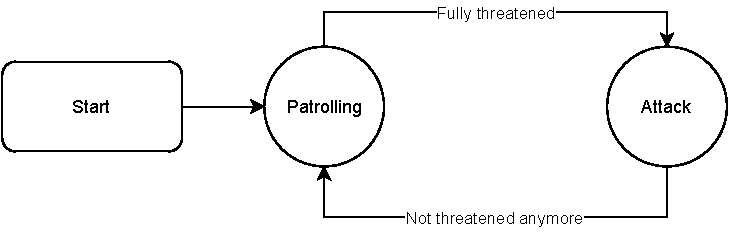
\includegraphics[width=0.6\textwidth]{figures/enemy_behaviour_states}
  \caption{Enemy behaviour state machine}
\end{figure}

Transitions between those two states are triggered by a single variable \varname{threat}. The threat level increases and decreases based on how far the player is from an enemy and for how much time.

Threatening is based on a fuzzy system, defined by the \varname{threat} value itself, \varname{onAlertThreshold} and \varname{attackThreshold}.

\begin{figure}[H]
  \centering
  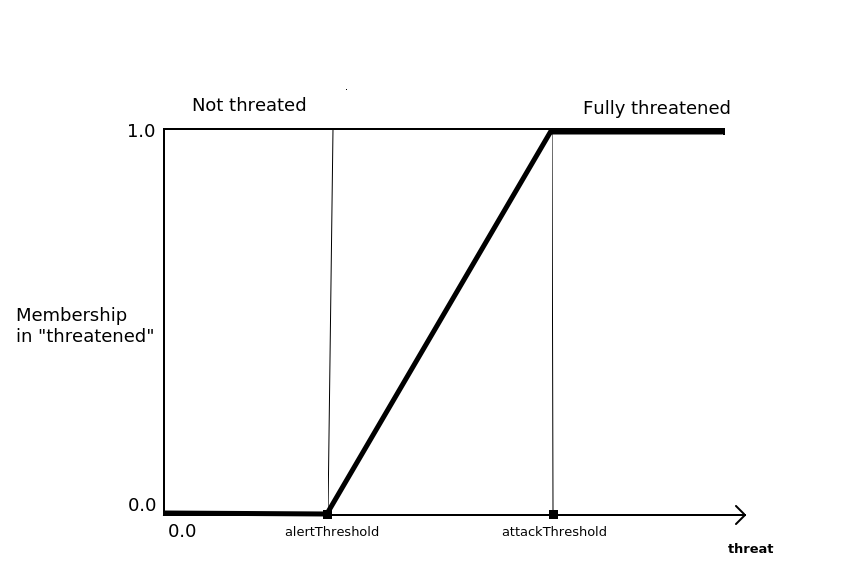
\includegraphics[width=0.8\textwidth]{figures/threat_graph}
  \caption{Threatening evaluation graph}
\end{figure}

As the \varname{threat} value grows, the enemy is first on guard and then starts attacking. When the \varname{threat} value goes down, the enemy stops chasing and resumes patrolling.

Note that if $alertThreshold < threat < attackThreshold$ the enemy's behaviour state doesn't change. While in this level, the enemy keeps active as before until one of the thresholds is hit.

\FloatBarrier

\begin{figure}
  \begin{lstlisting}
  procedure PatrolB positionehaviourUpdate():
      // Moves randomly around the current position
      PatrolArea() 

      if threat > attackThreshold:
        SetState(Attack)
  \end{lstlisting}
  \caption{Enemy patrolling state update pseudocode}
\end{figure}

\begin{figure}
  \begin{lstlisting}
    procedure AttackBehaviourUpdate():
      // Moves towards the player
      ChaseEntity(playerObject) 

      // If close enough to the player
      // attack him and reduce its HP
      if CloseTo(playerObject) and attackCooldown == 0: 
        Attack(playerObject)

      if threat < alertThreshold: 
        SetState(patrol)
  \end{lstlisting}
  \caption{Enemy attack state update pseudocode}
\end{figure}

\FloatBarrier

\subsection{Enemy evolution}
Enemies need to get stronger as the game progresses. To obtain this, a fixed number of enemies with random stats is instantiated \textit{(default = 10)} and stored in an object pool before the start of the game. The enemies in that pool are called \textit{offline} or resting enemies.

During the game, an enemy is on occasion extracted from the pool and spawned on the game field. Enemies present in the game world are called \textit{online} or spawned enemies. After these enemies are taken out of the game scene they go back to the offline pool.

This trick is already useful to improve performances as game objects are less likely to be created from scratch during the game, but the most interesting thing is that we can modify the offline enemies without any visible interruption of the gameplay.

\subsubsection{Stats}
Each enemy entity has different stats that evolve over time:

\begin{itemize}
  \item \textbf{Patrol speed} (\textit{patrolSpeed}): Movement speed while patrolling
  \item \textbf{Patrol zone size} (\textit{patrolZoneSize}): Size of the patrol zone
  \item \textbf{Patrol threat range} (\textit{patrolThreatRange}): Range from where the enemy is threatened by player's presence
  \item \textbf{Patrol threat growth} (\textit{patrolThreatGrowth}): The speed at which the threat value grows while patrolling
  \item \textbf{Patrol threat decay} (\textit{patrolThreatDecay}): The speed at which the threat value decreases while patrolling

  \item \textbf{Chasing speed} (\textit{chasingSpeed}): Movement speed while chasing the player
  \item \textbf{Attack range} (\textit{attackRange}): The minimum range to attack the player
  \item \textbf{Maximum chase range} (\textit{maximumChaseRange}): The maximum distance after which the enemy stops chasing the player
  \item \textbf{Attack damage} (\textit{attackDamage}): Damage dealt to the player after an attack
  \item \textbf{Maximum attack cooldown} (\textit{maxAttackCooldown}): The cooldown time between two consecutive attacks
  \item \textbf{Attack threat growth} (\textit{attackThreatGrowth}): The speed at which the threat value grows while attacking
  \item \textbf{Attack threat decay} (\textit{attackThreatDecay}): The speed at which the threat value decreases while attacking
\end{itemize}

These values are considered the \textit{genes} of the enemy as they define how \textit{strong} an enemy is. The \textit{strength} of an enemy is based on part of its stats and is evaluated using the below formula:

\begin{gather*}
  strength(foe) =
    foe.patrolSpeed + \\
    foe.patrolZoneSize + \\
    foe.patrolThreatRange + \\
    foe.hasingSpeed + \\
    foe.attackRange + \\
    foe.maximumChaseRange + \\
    \frac{foe.attackDamage}{5} + \\
    \frac{2}{foe.maxAttackCooldown}
\end{gather*}

\pagebreak

\subsubsection{Breeding}
The \textit{breeding} phase involves two different enemies and produces a child which stats are the result of taking the best stats of both parents and mixing them together.
This approach ensures that a child will always be at least as strong as the parents, making the game rapidly more difficult in the progress.

\begin{figure}[H]
  \begin{lstlisting}
  procedure Breed(parent1, parent2):
    child = CreateEmptyEnemy()

    if strength(parent1) > strength(parent2):
      child.kind = parent1.kind
    else:
      child.kind = parent2.kind

    foreach stat_var in child:
      child.stat_var = max(parent1.stat_var, parent2.stat_var)

    return child 
  \end{lstlisting}
  \caption{Breeding procedure pseudocode}
\end{figure}

\subsubsection{Mutations}
There’s always a chance that during breeding the child genes mutate, leading to a completely different result than what’s expected. When a child mutates, its type and its genes are generated randomly again instead of being derived from the parents. The type is chosen from any possible types, but the weaker enemy types stop spawning after a period of time to ensure that while the game progresses, new types of enemies are present, and that the difficulty doesn’t decrease. The genes are initialized randomly such as when the initial population is instantiated at the start of the game.

Note that a mutation doesn’t assure that the resulting enemy will be stronger or equal to the parents, nor that it will be of a stronger kind. The trend of the strength of spawned enemies is not monotonic, but tends to grow over time.

\subsubsection{Genetic selection overview}
The genetic selection step is executed in fixed intervals of time and involves only offline enemies. As it replaces a consistent number of entities it requires the offline pool to be big enough, otherwise the step is skipped.

Enemies present in the pool are sorted by their strength and worst pairs of enemies are popped out. The best enemies are bred to generate two new children, while worst two are destroyed and replaced by two brand new enemies of the weakest type possible with randomly generated stats.

\begin{figure}[H]
  \begin{lstlisting}
  procedure GeneticSelectionStep():
    SortByStrength(offlineEnemies)

    topEnemy1 = PopFromTop(offlineEnemies)
    topEnemy2 = PopFromTop(offlineEnemies)

    worstEnemy1 = PopFromBottom(offlineEnemies)
    worstEnemy2 = PopFromBottom(offlineEnemies)

    // Breed top enemies
    // Note that mutations can occur in this phase on both
    // of the calls of Breed()
    Push(offlineEnemies, Breed(topEnemy1, topEnemy2))
    Push(offlineEnemies, Breed(topEnemy2, topEnemy1))

    // Replace worst enemies with new ones
    Push(offlineEnemies, GenerateNewEnemy())
    Push(offlineEnemies, GenerateNewEnemy())
  \end{lstlisting}
  \caption{Genetic selection step procedure pseudocode}
\end{figure}

Not all offline enemies are involved in breeding. Some remain in the pool as they are and will be involved in mating/replacing in subsequent steps.

It may be possible to create a bigger pool and use more pairs during genetic selection. However, the approach shown above requires little computational power and still gives good results in terms of the game progression.

\subsubsection{Literature references and further readings}

The enemy behaviour approach was highly inspired by the concepts of \textit{fuzzy logic} developed by Lofti Zadeh (1921-2017) and proposed as an application in its 1973 paper \textit{"Outline of a new approach to the analysis of complex systems and decision processes"} from \textit{IEEE Trans. Systems, Man and Cybernetics, 1973; 3: 28–44}. Although using a single variable doesn't express the full power of fuzzy systems, the results were good enough to not make the enemy behaviour more complex than it already is.

The enemy evolution algorithm is based on the theory of \textit{Genetic algorithms} by John Holland (1929-2015) during the '60s and extensively described in \textit{Adaptation in Natural and Artificial Systems (1975, MIT Press)}, which is considered the killer book on genetic algorithms. As the game theme is about mutations and species evolution, this approach was literally the first that came in mind while planning down the enemies system.

The level generation algorithm was inspired by the demonstration material from Week 9 of the course.

\section{Conclusions}
\subsection{Team role}
\subsubsection{Lorenzo Catania}
I've made my part on the game development as a game script programmer,gameplay designer and sound/FX and music composer.

\subsubsection{Malcolm Grech}
My role in the game development was as a mostly as a backend developer with some frontend jobs.

\subsubsection{Francesco Borg Bonello}

I had the role as team leader with overall contribution to both frontend and backend.

\subsection{Personal contributions}
\subsubsection{Lorenzo Catania}
I've designed and implemented the camera movement controller, the entities garbage collection and most of all the enemy spawning, evolution and behaviour.

I've partecipated in designing and tuning the level generation and the score system.

I've edited the FX sounds, but none of them was originally created by me.

I've also composed the menu background music, trivially titled \textit{Deep Blue menu song}.

\subsubsection{Malcolm Grech}
My contribution to the game development where:
Creating the Menu scene Management and button/scroller functionality.
A part in the creation of the player movement and camera controller.
Creating the level generation which was fine tuned with other later additions.

\subsubsection{Francesco Borg Bonello}

Apart from overall team management as team leader, my role was creating the player survivability script along with the score system, creating the pickup system, implementing fuzzy logic in the game objects, handling all the UI, implementing the animations and sound and also fine tuning the Genetic Algorithm with Lorenzo as well as player movement.

\subsection{Final thoughts}
\subsubsection{Lorenzo Catania}
I would like to say thanks to everyone that has permitted this beatiful experience, first of all my whole team that worked wonderfully without any stops during the 2 days of the jam. Thanks also to University of Malta and its lecturers for guiding me in its new experience, as well as GDG Malta, MITA and all of the organizers of the event. Thanks to the catering as well, that was pretty good throughout all the weekend.

\subsubsection{Malcolm Grech}
The experience of my first gameJam was an extremely satisfying and enjoyable one. Having been allocated time to focus on creating a source of entertainment with a team of other capable creators was an honour. My only displeasures where my lack of connecting to my teammates, as my work was on occasion undermined and taken over. Though I had made significant contributions to the game development, I feel like I could have done better, and pushed more till the end as I plan to do in future Jams.

\subsubsection{Francesco Borg Bonello}
I feel that this tiring weekend was fruitful in terms of what I learnt and experienced. I would like to say thank you to all those involved in organizing the event and most importantly my teammates for the swift collaboration throughout. I am sure the rest of the team is equally as proud as I am for ultimately winning this year's Game Jam!

\end{document}